% =====================================================
\chapter{Foundational Experiments}
\label{chap:foundational_experiments}

This chapter presents a series of foundational experiments conducted to build an intuitive understanding of the key components that drive diffusion-based generative models.  
The intent was not to reproduce benchmark-level results but to practically observe how different architectures behave once trained, i.e., how the loss evolves, how reconstruction emerges from noise, and how various conditioning mechanisms influence the generation process.  
The experiments focused on the Vision Transformer (ViT)~\cite{dosovitskiy2020vit}, the U–Net backbone~\cite{ronneberger2015unet}, the Denoising Diffusion Probabilistic Model (DDPM)~\cite{ho2020ddpm}, and the Conditional Diffusion framework with classifier-guided generation~\cite{ho2020ddpm,radford2021clip}.  
Together, they form the conceptual and empirical foundation upon which later adaptive and style-aware diffusion experiments are built.

Each experiment captures one essential property of diffusion systems: ViT illustrates the power of attention in capturing global context; U–Net demonstrates how spatial structure is preserved through skip connections; DDPM visualizes the transformation from noise to structure; and classifier-guided diffusion introduces controllability through explicit gradient-based conditioning.

% =====================================================
\section{Vision Transformer (ViT) Experiments}
\label{sec:vit_experiments}

The Vision Transformer (ViT)~\cite{dosovitskiy2020vit} experiment was designed to understand how transformer-based vision models capture global relationships in images compared to convolutional architectures.  
A compact ViT with a shallow DETR-style~\cite{carion2020endtoendobjectdetectiontransformers} head was implemented to explore how patch embeddings interact with query-based decoding.  
Training was performed on CIFAR-10, with images resized to \(224\times224\) to fit the patch embedding scheme.  
The setup used the Adam optimizer (\(3\times10^{-4}\)), batch size 64, and 50 epochs of training with ReLU activation and 0.1 dropout.  
The network used a 768-dimensional embedding space, 12 attention heads, and a patch size of 16.

DETR (Detection Transformer)~\cite{carion2020endtoendobjectdetectiontransformers} was originally introduced to remove handcrafted detection stages such as anchor boxes or non-maximum suppression, relying solely on attention to perform end-to-end object detection.  
It formulates detection as a direct set prediction task using the Hungarian loss for optimal bipartite matching between predicted and ground-truth objects.  
In this experiment, while detection itself was not the goal, integrating the DETR-style decoder provided a practical view of how attention can align semantically meaningful tokens, thereby learning structure without explicit convolution.

\paragraph{Results}
The ViT achieved around \textbf{85\% test accuracy} on CIFAR-10.  
Attention visualizations clearly revealed that transformer heads concentrated on key object parts (e.g., airplane wings or vehicle bodies) while ignoring background clutter.  
Training was smooth, with stable convergence by the 40th epoch.  
The experiment reinforced the interpretability and global reasoning capacity of attention, thereby forming the mental framework used later to understand cross-attention in diffusion models.  

\begin{figure}[!h]
    \centering
    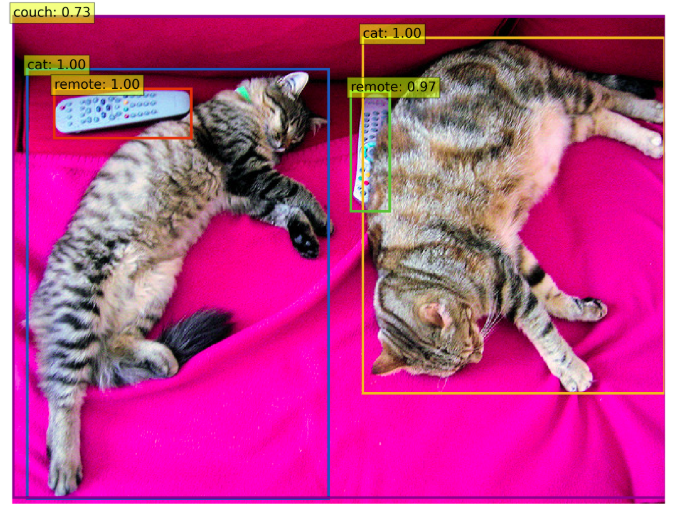
\includegraphics[width=0.65\linewidth]{images/vit_results.png}
    \caption{Vision Transformer on CIFAR-10: attention heads highlighting key semantic regions.}
    \label{fig:vit_results}
\end{figure}

% =====================================================
\section{U–Net Backbone Experiments}
\label{sec:unet_experiment}

Next, the U–Net~\cite{ronneberger2015unet} backbone was explored to understand how skip connections preserve fine structure during reconstruction, a feature that makes it the default denoising network in diffusion models.  
A basic U–Net autoencoder was trained on the Oxford-IIIT Pet dataset (\(128\times128\) resolution) for segmentation using Adam (\(1\times10^{-3}\)), cross-entropy loss, and batch size 8.  
Each encoder block contained two \(3\times3\) convolutions with ReLU followed by max pooling; the decoder mirrored this with transposed convolutions and symmetric skip connections.  
The architecture was intentionally kept simple to focus on reconstruction behavior rather than architectural sophistication.

\paragraph{Results}
Training converged quickly, with the model accurately recovering spatial boundaries after just a few epochs.  
Figure~\ref{fig:unet_segmentation_results} shows clean, sharp segmentation outputs that closely match ground-truth masks.  
Skip connections clearly restored high-frequency information lost during downsampling, which explains why the same structure works so effectively in denoising networks.  
In diffusion settings, these skip pathways combine with sinusoidal time-step embeddings, thereby giving the model temporal awareness of which stage of denoising it is in and making U–Net both spatially and temporally adaptive.

\begin{figure}[!h]
    \centering
    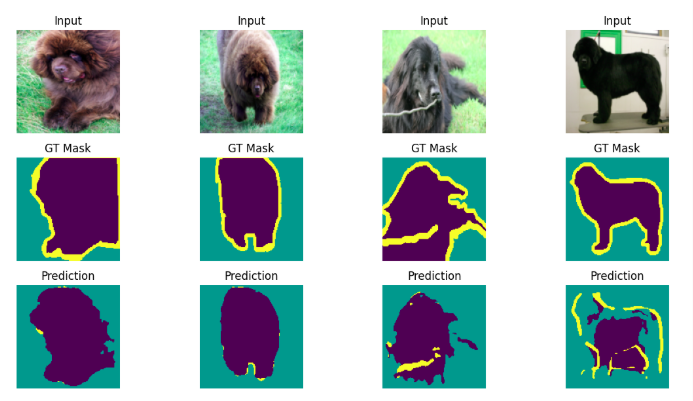
\includegraphics[width=0.55\linewidth]{images/unet_segmentation_results.png}
    \caption{U–Net on Oxford-IIIT Pet: input, ground truth, and reconstructed output.}
    \label{fig:unet_segmentation_results}
\end{figure}

% =====================================================
\section{Denoising Diffusion Probabilistic Model (DDPM)}
\label{sec:ddpm_experiments}

% The DDPM~\cite{ho2020ddpm} experiment visualized the “order from noise” process central to diffusion-based generation.  
% The U–Net architecture was reused here, augmented with sinusoidal time embeddings to inject temporal information.  
% Training was done on MNIST(resized to \(32\times32\)) for 15 epochs, with Adam (\(1\times10^{-4}\)) and 1000 diffusion steps using a linear \(\beta_t\) schedule between \(1\times10^{-4}\) and \(2\times10^{-2}\).  
% The model learned to predict the clean image \(x_0\) from a noisy sample \(x_t\) by minimizing MSE between predicted and actual noise.

% \paragraph{Results}
% The generated results demonstrated the expected diffusion progression: early steps resembled pure Gaussian noise; mid-steps revealed faint outlines; final stages formed crisp, legible digits.  
% This directly validated the theoretical denoising process.  
% The model produced consistent and interpretable transitions, providing an intuitive feel for how diffusion learns to reverse noise step by step and construct order through learned probabilistic transitions.
\noindent
The DDPM~\cite{ho2020ddpm} experiment visualized the \emph{“order from noise”} process central to diffusion-based generation.  
A U–Net backbone was employed, augmented with sinusoidal time embeddings to encode temporal information.  
Training was performed on MNIST (resized to \(32\times32\)) for 15 epochs using the Adam optimizer (\(1\times10^{-4}\)) and a linear \(\beta_t\) schedule ranging from \(1\times10^{-4}\) to \(2\times10^{-2}\) over 1000 diffusion steps.  
The network learned to predict the clean image \(x_0\) from a noisy latent \(x_t\) by minimizing mean-squared error between the predicted and actual noise.

\paragraph{Results.}
Figure~\ref{fig:ddpm_samples} illustrates the progressive refinement of generated digits.  
At the earliest diffusion steps, outputs resemble pure Gaussian noise with no discernible structure.  
As sampling proceeds, faint digit contours appear i.e a reflection of the model beginning to estimate global shape information.  
Midway through the denoising trajectory, the model stabilizes coarse structure (loops of 0, stalks of 1 or 9), while fine pixel-level details remain stochastic.  
In the final few steps, residual noise is systematically removed, revealing sharply formed digits with clear boundaries and correct topology.  

This progression provides an intuitive visualization of how diffusion models learn to reverse entropy: rather than generating pixels directly, the model gradually transforms a noise distribution into structured data through a sequence of learned conditional transitions.  
The experiment also highlights the smooth and interpretable nature of diffusion learning  unlike GANs~\cite{goodfellow2014gan}, where generation can be abrupt or unstable, diffusion exhibits continuous improvement across time steps, offering clear insight into how the model internalizes spatial and probabilistic cues from the dataset.  
Despite being trained on a simple dataset (MNIST), the experiment effectively demonstrates the fundamental mechanics of diffusion, validating the theoretical framework that underpins more advanced models such as Stable Diffusion and InstantStyle.

\begin{figure}[!h]
    \centering
    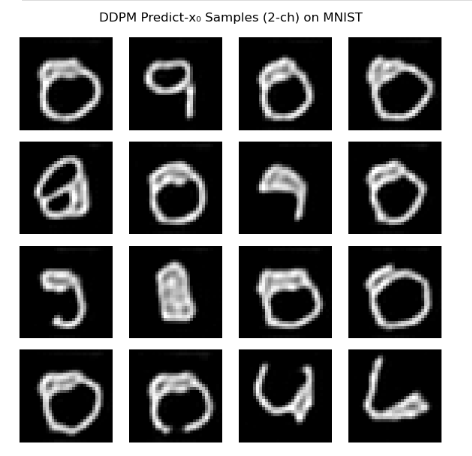
\includegraphics[width=0.65\linewidth]{images/ddpm_samples.png}
    \caption{DDPM on MNIST: progressive denoising from pure noise to clear digits.}
    \label{fig:ddpm_samples}
\end{figure}

% =====================================================
\section{Conditional Diffusion (Classifier-Guided)}
\label{sec:conditional_diffusion_experiments}

Finally, the classifier-guided diffusion setup introduced explicit control into the generative process.  
A DDPM denoiser was paired with a CNN~\cite{oshea2015introductionconvolutionalneuralnetworks} classifier trained on noisy MNIST samples to predict class labels at varying noise levels (Adam \(1\times10^{-3}\), batch size 128, 10 epochs).  
During sampling, gradients from \(\nabla_{x_t}\log p_\phi(y|x_t)\) were added to the DDPM mean estimate, scaled by a guidance factor \(\lambda=2.0\), thereby steering generation toward the specified target class.

\paragraph{Results}
At lower guidance scales, the model generated diverse samples, whereas higher \(\lambda\) values produced sharper and more class-consistent digits at the cost of variety.  
The results visually confirmed that classifier gradients can effectively modulate diffusion trajectories, which is a precursor to modern conditioning mechanisms such as cross-attention.  
This small but powerful experiment completed the conceptual bridge between unconditioned diffusion and controlled, prompt-driven generation.

\begin{figure}[!h]
    \centering
    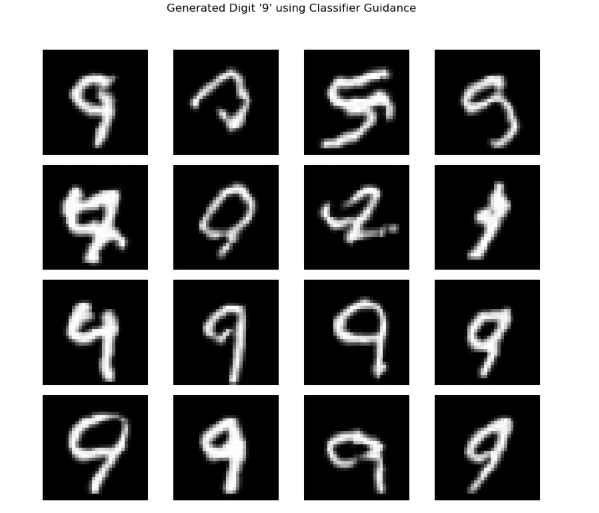
\includegraphics[width=0.65\linewidth]{images/guided_diffusion_results.png}
    \caption{Classifier-Guided Diffusion on MNIST: class “9” generations at guidance scale \(\lambda=2.0\).}
    \label{fig:guided_diffusion_results}
\end{figure}

% =====================================================
\section{Summary of Foundational Experiments}
\label{sec:foundational_summary}

The foundational experiments provided a cohesive understanding of the mechanisms behind diffusion-based image generation.  
The Vision Transformer~\cite{dosovitskiy2020vit} showed how attention captures long-range context, the U–Net~\cite{ronneberger2015unet} demonstrated spatial reconstruction, and the DDPM~\cite{ho2020ddpm} revealed structure emerging from noise, while conditional diffusion established controllability through gradient-based guidance.  
Together, these results grounded the theory and laid the foundation for exploring style-aware and adaptive diffusion frameworks such as StyleShot~\cite{gao2024styleshot}, CSGO~\cite{xing2024csgocomp}, InstantStyle~\cite{wang2024instantstyle}, InstantStyle-Plus~\cite{wang2024instantstyleplus}, and the proposed CSD~\cite{somepalli2024csd}-guided architecture.
